\documentclass[12pt , a4paper]{article}

\usepackage[french]{babel}
\usepackage [utf8] {inputenc} % utf-8 / latin1
\usepackage[T1]{fontenc}
\usepackage{aeguill} %impression de qualite des listings
\usepackage {amsmath}
\usepackage {mathpazo}
\usepackage {hyperref} %lien dynamique
\usepackage {graphicx}%image
\usepackage {fancyhdr}%entete et pied de page
\usepackage {float} %image
\usepackage {color}
\usepackage{lastpage}
\usepackage[top=2cm, bottom=2cm, left=2cm , right=2cm]{geometry}
\usepackage{vmargin}
\usepackage{listings}
\usepackage{lscape}


\definecolor{hellgelb}{rgb}{1,1,0.8}
\definecolor{colKeys}{rgb}{0,0,1}
\definecolor{colIdentifier}{rgb}{0,0,0}
\definecolor{colComments}{rgb}{0,0.5,0}
\definecolor{colString}{rgb}{0.62,0.12,0.94}

\newcommand {\TitreCours}{Java distribué}
\newcommand {\Epoque}{GM4 - 2ème semestre}
\newcommand {\Prof}{M. Pécuchet}
\newcommand {\Auteur}{Pauline Réquéna \and Guillaume Dubuisson Duplessis}

\newcommand{\J}{
  \lstset{
    language=java,
    float=hbp,
    basicstyle=\ttfamily\small,
    identifierstyle=\color{colIdentifier},
    keywordstyle=\bf \color{colKeys},
    stringstyle=\color{colString},
    commentstyle=\color{colComments},
    columns=flexible,
    tabsize=5,
    frame=single,
    % frame=shadowbox,
    rulesepcolor=\color[gray]{0.5},
    extendedchars=true,
    showspaces=false,
    showstringspaces=false,
    numbers=left,
    stepnumber=5,
    firstnumber=1,
    numberstyle=\tiny,
    breaklines=true,
    % backgroundcolor=\color{hellgelb},
    captionpos=b,%
  }
}


\title{Java distribué\\
  \vspace{0.6cm}
  \normalsize{Gestionnaire d'agendas} 
  \begin{center}
    % \includegraphics[scale=3.5]{./images/piton3d.jpg}
  \end{center}
}
\author{\Auteur}
\date{\today}

% UNE METHODE DE DEFINITION D'ENTETE
% \pagestyle{fancy}
% \fancyhf{}%detruit les entetes deja presents
% \renewcommand{\headrulewidth}{0.4pt}
% \renewcommand{\footrulewidth}{0.4pt}
% \lhead{\Auteur}
% \rhead{\today}
% \rfoot{\thepage\ sur \pageref{LastPage}}

% MEMO
% \lhead{haut gauche}
% \chead{centre haut}
% \rhead{haut droit}
% \lfoot{bas gauche}

% UNE AUTRE METHODE
% \pagestyle{headings}
\setmarginsrb{2.5cm}{1cm}{1cm}{1.5cm}{.5cm}{.5cm}{.5cm}{.5cm}
% \renewcommand{\sectionmark}[1]{\markright{\textsc{\TitreCours:} \thesection. \#1 \hrulefill\ \textup{page }}}
% FONCTIONNEMENT DE \setmarginsrb
% \setmarginsrb{1}{2}{3}{4}{5}{6}{7}{8}
% 1 est la marge gauche
% 2 est la marge en haut
% 3 est la marge droite
% 4 est la marge en bas
% 5 fixe la hauteur de l'entête
% 6 fixe la distance entre l'entête et le texte
% 7 fixe la hauteur du pied de page
% 8 fixe la distance entre le texte et le pied de page

% UNE DERNIERE METHODE
\pagestyle{fancy}
\fancyhf{}%supprime les entetes et pieds de page utilise par defaut par LaTeX
% \rightmark : contient le nom de la section courante
% \markright : contient le nom de la section courante
% \renewcommand{\sectionmark}[1]{\markright{\#1}}
% \renewcommand{\chaptermark}[1]{\markboth{\bsc{\chaptername~\thechapter{} :} #1}{}}
\renewcommand{\sectionmark}[1]{\markright{\thesection{} #1}}
\lhead[\thepage]{\TitreCours\ - \rightmark} 
\rhead{\Epoque}
\rfoot{\thepage\ / \pageref{LastPage}}

\fancypagestyle{plain}{ 
  \fancyhead{} 
  \renewcommand{\headrulewidth}{0pt}
}

\begin{document}
\maketitle
\thispagestyle{empty}
% \setcounter{page}{0}
\newpage
\thispagestyle{plain}% page sans entete 

\tableofcontents
\newpage
\section{Introduction}
\noindent blabla

\newpage
\section{Analyse détaillée du sujet}

\subsection{Description du sujet}
Le sujet de notre mini-projet de Java Distribu\'e consiste en la
conception et l{\textquoteright}impl\'ementation d{\textquoteright}un
site web de gestion d{\textquoteright}agendas. Ce site a pour fonction
de g\'erer les diff\'erents types d{\textquoteright}agendas
d{\textquoteright}un utilisateur. Par exemple, un utilisateur peut
disposer d{\textquoteright}un agenda
{\guillemotleft}~Travail~{\guillemotright} pour ses rendez-vous
professionnels et d{\textquoteright}un agenda
{\guillemotleft}~Perso~{\guillemotright} pour ses activit\'es
personnelles. Cette application permettra donc la gestion individuelle
de ces 2 agendas.


\vspace{0.5cm}

\noindent Un utilisateur de ce gestionnaire devra donc pouvoir~avoir acc\`es aux
fonctionnalit\'es suivantes :


\begin{itemize}
\item \textbf{Consulter ses agendas sous une forme claire et
    fonctionnelle}
\end{itemize}
Nous avons opt\'e pour l{\textquoteright}affichage des agendas par
semaine. Par ailleurs, afin de pouvoir bien distinguer les diff\'erents
agendas lors de l{\textquoteright}affichage des \'ev\`enements, chaque
agenda est caract\'eris\'e par une couleur.

\vspace{0.5cm}
\begin{itemize}
\item \textbf{Cr\'eer un nouvel agenda}
\end{itemize}
Un agenda est caract\'eris\'e par un nom, un lieu
d{\textquoteright}application, une description, ainsi
qu{\textquoteright}une couleur.

\vspace{0.5cm}
\begin{itemize}
\item \textbf{Modifier les param\`etres d{\textquoteright}un agenda
    pr\'eexistant}
\end{itemize}
Une fois qu{\textquoteright}un agenda a \'et\'e cr\'ee,
l{\textquoteright}utilisateur doit pouvoir s{\textquoteright}il le
souhaite en modifier les d\'etails ou la couleur
d{\textquoteright}affichage.

\vspace{0.5cm}
\begin{itemize}
\item \textbf{Supprimer un agenda pr\'eexistant}
\end{itemize}
Lorsqu{\textquoteright}un agenda n{\textquoteright}est plus utilis\'e
par l{\textquoteright}internaute, celui-ci peut le supprimer, afin de
ne pas encombrer son compte de donn\'ees inutiles. Ce
n{\textquoteright}est pas une action anodine, car toute suppression est
irr\'eversible et entra\^ine la suppression de tous \'ev\`enements de
l{\textquoteright}agenda.

\vspace{0.5cm}
\begin{itemize}
\item \textbf{Cr\'eer un nouvel \'ev\`enement dans un agenda
    pr\'eexistant}
\end{itemize}
Un \'ev\`enement appartient \`a un agenda. Il est caract\'eris\'e par un
objet, une date, un lieu, des heures de d\'ebut et de fin, ainsi
qu{\textquoteright}une description.

\vspace{0.5cm}
\begin{itemize}
\item \textbf{Modifier les caract\'eristiques d{\textquoteright}un
    \'ev\`enement pr\'eexistant}
\end{itemize}
Une fois qu{\textquoteright}un \'ev\`enement a \'et\'e cr\'ee dans un
agenda, l{\textquoteright}utilisateur doit pouvoir s{\textquoteright}il
le souhaite en modifier les d\'etails.

\vspace{0.5cm}
\begin{itemize}
\item \textbf{Supprimer un \'ev\`enement pr\'eexistant}
\end{itemize}






\subsection{Structure du site}


L{\textquoteright}acc\`es \`a ce site se fera par le biais
d{\textquoteright}une page d{\textquoteright}authentification. En
effet, les comptes de chaque utilisateur sont confidentiels. Pour se
connecter au gestionnaire d{\textquoteright}agendas,
l{\textquoteright}internaute devra donc en premier lieu saisir son
login et son mot de passe.

\vspace{0.5cm}

\noindent Une fois l{\textquoteright}authentification accomplie,
l{\textquoteright}internaute sera dirig\'e vers la page
d{\textquoteright}accueil, compos\'ee de plusieurs parties :


\begin{itemize}
\item \textbf{L{\textquoteright}en-t\^ete}
\end{itemize}
Elle est constitu\'ee du logo de l{\textquoteright}application,
d{\textquoteright}un message d{\textquoteright}accueil et du bouton de
d\'econnexion.

\vspace{0.5cm}
\begin{itemize}
\item \textbf{Le menu de gauche~}
\end{itemize}
Ce menu est compos\'e tout d{\textquoteright}abord de la liste des
agendas de l{\textquoteright}utilisateur connect\'e. Ce dernier peut
s\'electionner dans cette liste les agendas qu{\textquoteright}il
d\'esire ou non afficher.

\noindent A travers ce menu, l{\textquoteright}utilisateur peut \'egalement
acc\'eder aux diff\'erentes fonctionnalit\'es de gestion des agendas,
\`a savoir la cr\'eation d{\textquoteright}un nouvel agenda, la
modification ou la suppression d{\textquoteright}un agenda, ainsi que
la cr\'eation d{\textquoteright}un nouvel \'ev\`enement. La
modification ou la suppression d{\textquoteright}un \'ev\`enement se
fera par le biais du calendrier d{\textquoteright}affichage.

\vspace{0.5cm}
\begin{itemize}
\item \textbf{Le corps de la page}
\end{itemize}
Il est compos\'e du tableau d{\textquoteright}affichage des agendas. En
cliquant sur un des \'ev\`enements affich\'e sur ce calendrier,
l{\textquoteright}utilisateur pourra en modifier les d\'etails, ou le
supprimer.



L{\textquoteright}affichage des agendas \'etant hebdomadaire,
l{\textquoteright}utilisateur pourra passer d{\textquoteright}une
semaine \`a l{\textquoteright}autre \`a l{\textquoteright}aide de
fl\`eches directionnelles.

\subsection{Aspects techniques}

\begin{itemize}
\item Le planning de ce projet sera r\'ealis\'e sur le logiciel
  GanttProject.
\item La mod\'elisation et le d\'eveloppement de ce projet seront
  effectu\'es sur l{\textquoteright}IDE Netbeans 6.5.
\item Les interfaces des diff\'erentes pages web seront r\'ealis\'ees en
  xHTML/CSS.
\item Des JSP permettront d{\textquoteright}ins\'erer des donn\'ees
  dynamiques \`a ce contenu statique.
\item Les informations enregistr\'ees dans l{\textquoteright}application
  seront stock\'ees dans une base de donn\'ees MySQL et la liaison de
  l{\textquoteright}application \`a la base se fera via une connexion
  JDBC.
\end{itemize}

\subsection{Diagramme de Gantt du mini-projet}
	\begin{center}
	  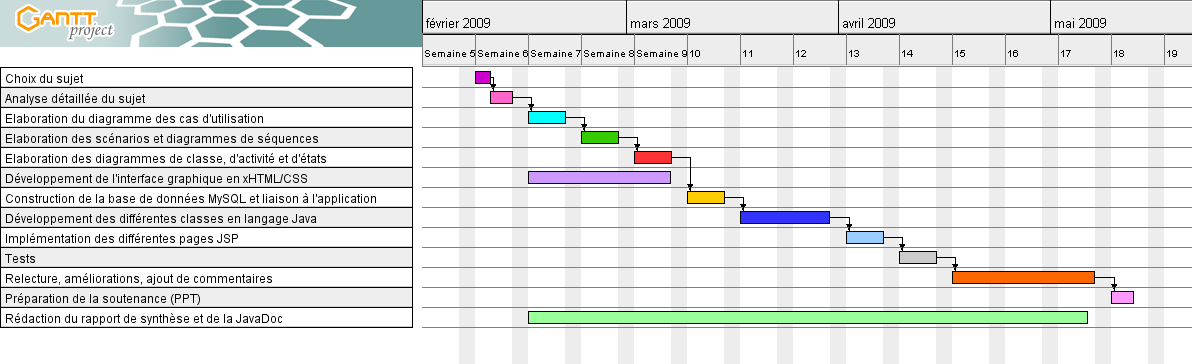
\includegraphics[scale=0.4]{./images/planning_projet_JAVA.png}
	\end{center}
	\begin{center}
	  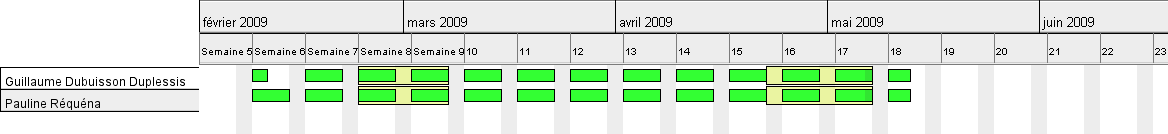
\includegraphics[scale=0.4]{./images/planning_projet_JAVA_res.png}
	\end{center}

\newpage
\section{Cas d'utilisation}
\subsection{Identification des acteurs}
Dans le cadre de  ce gestionnaire d'agendas, nous pouvons déterminer deux  principaux acteurs : l'utilisateur "lambda" qui gère  ses agendas et l'administrateur du site. Dans  un soucis de simplicité,
nous ne développerons pas l'administration du site. Nous ne considérerons donc pas l'administrateur.
\subsection{Diagramme de cas d'utilisation}
	\begin{center}
	  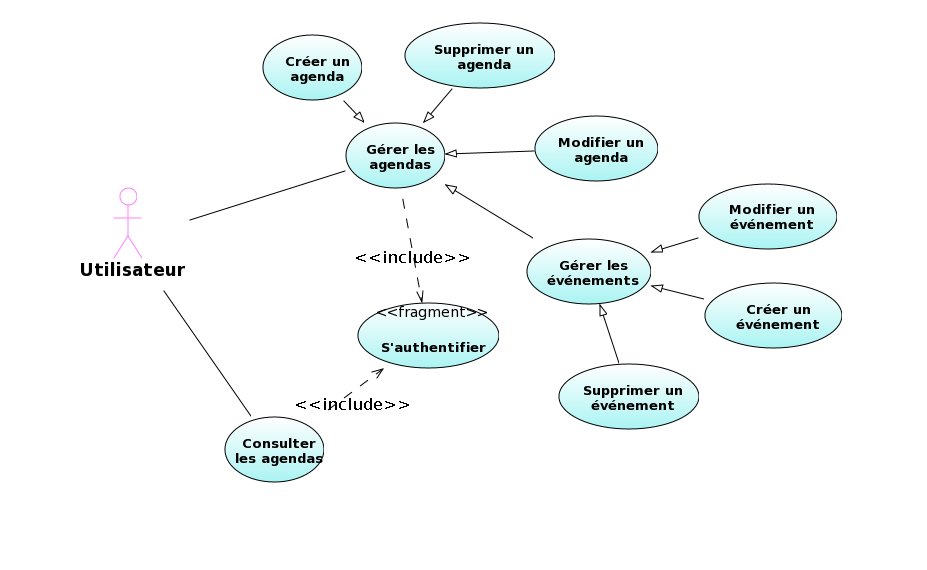
\includegraphics[scale=0.6]{./images/use_cases.png}
	\end{center}
\noindent Nous pouvons remarquer qu'il  n'apparaît pas de scénario d'inscription au site internet. En effet,  nous préférons nous concentrer sur la gestion des agendas  en elle-même que sur la gestion
des membres.

\subsection{Les scénarios détaillés}
\subsubsection{Scénario "s'authentifier"}

\noindent\textbf{Titre : } s'authentifier\\
\textbf{Résumé : } ce cas d'utilisation permet à l'utilisateur de s'authentifier\\
\textbf{Acteur : }utilisateur\\

\noindent\textbf{Préconditions :}
\begin{itemize}
\item L'utilisateur n'est pas déjà authentifié
\item La base de données stockant la liste utilisateur/mot de passe est accessible \\
\end{itemize}


\noindent\textbf{Scénario nominal :}
\begin{enumerate}
\item Le système demande à l'utilisateur un nom d'utilisateur et un mot de passe
\item L'utilisateur indique son nom d'utilisateur et son mot de passe
\item Le système vérifie qu'un utilisateur correspond au nom d'utilisateur
\item Le système vérifie que le mot de passe indiqué correspond au mot de passe associé au nom de l'utilisateur
\item Le système crée une session pour l'utilisateur \\
\end{enumerate}


\noindent\textbf{Encha\^inements alternatifs :}\\
\noindent\textit{A1 : nom d'utilisateur provisoirement erroné}\\
L'encha\^inement A1 démarre au point 3 du scénario nominal.
\begin{enumerate}
\item[4.] Le système indique à l'utilisateur que le nom d'utilisateur est erroné pour la première ou la deuxième fois
\item[5.] Le système incrémente le compteur des tentatives d'authentification
\end{enumerate}
Le scénario nominal reprend au point 1.\\


\noindent\textit{A2 : mot de passe provisoirement erroné}\\
L'encha\^inement A2 démarre au point 4 du scénario nominal.
\begin{enumerate}
\item[5.] Le système indique à l'utilisateur que le mot de passe est erroné pour la première ou la deuxième fois
\item[6.] Le système incrémente le compteur des tentatives d'authentification
\end{enumerate}
Le scénario nominal reprend au point 1.\\


\noindent\textbf{Encha\^inements d'erreur :}\\
\noindent\textit{E1 : nom d'utilisateur définitivement erroné}\\
L'encha\^inement E1 démarre au point 3 du scénario nominal.
\begin{enumerate}
\item[4.] Le système indique à l'utilisateur que le nom d'utilisateur est erroné pour la 3ème fois
\item[5.] Le système indique que toute tentative d'authentification sera refusée
\item[6.] Le système enregistre la machine comme étant bannie pour une durée déterminée (par exemple 1h)
\end{enumerate}


\noindent\textit{E2 : mot de passe définitivement erroné}\\
L'encha\^inement E2 démarre au point 4 du scénario nominal.
\begin{enumerate}
\item[5.] Le système indique à l'utilisateur que le mot de passe est erroné pour la 3ème fois
\item[6.] Le système indique que toute tentative d'authentification sera refusée
\item[7.] Le système enregistre la machine comme étant bannie pour une durée déterminée (par exemple 1h)
\end{enumerate}


\subsubsection{Scénario "Création d'un nouvel agenda"}

\noindent\textbf{Titre : } Création d’un nouvel agenda\\
\textbf{Résumé : } Ce scénario permet à l’utilisateur de créer un nouvel agenda dans son calendrier.\\
\textbf{Acteur : }utilisateur\\

\noindent\textbf{Préconditions :}
\begin{itemize}
\item L'utilisateur est authentifié
\item La base de données stockant la table des agendas est accessible\\
\end{itemize}


\noindent\textbf{Scénario nominal :}
\begin{enumerate}
\item L’utilisateur indique qu'il souhaite créer un nouvel agenda 
\item Le système affiche le formulaire de création d’agendas.
\item L'utilisateur renseigne le formulaire avec le nom de l'agenda, le lieu, une description, et une couleur représentative
\item Le système vérifie que le champ "Nom" est bien renseigné
\item Le système vérifie qu’aucun agenda du même nom n’existe déjà dans la base
\item Le système crée un nouvel agenda dans la base de données.\\
\end{enumerate}


\noindent\textbf{Encha\^inements alternatifs :}\\
\noindent\textit{A1 : le champ nom est vide}\\
L'encha\^inement A1 démarre au point 4 du scénario nominal.
\begin{enumerate}
\item[5.] Le système indique à l’utilisateur que le champ « Nom » n’est pas rempli et que la création est donc impossible.
\end{enumerate}
Le scénario nominal reprend au point 2.\\


\noindent\textit{A2 : il y a déjà un agenda du même nom dans la base}\\
L'encha\^inement A2 démarre au point 5 du scénario nominal.
\begin{enumerate}
\item[6.] Le système indique à l’utilisateur que ce nom est déjà utilisé et qu’il doit en choisir un nouveau.
\end{enumerate}
Le scénario nominal reprend au point 2.\\


\subsubsection{Scénario "Modifier les paramètres d'un agenda"}
\noindent\textbf{Titre : } Modification d’un agenda\\
\textbf{Résumé : } Ce scénario permet à l’utilisateur de modifier les caractéristiques d’un agenda existant, s’il veut par exemple changer sa couleur ou son nom.\\
\textbf{Acteur : }utilisateur\\

\noindent\textbf{Préconditions :}
\begin{itemize}
\item L’utilisateur est authentifié
\item L'agenda doit exister
\item La base de données stockant la table des agendas est accessible\\
\end{itemize}


\noindent\textbf{Scénario nominal :}
\begin{enumerate}
\item L’utilisateur indique qu'il souhaite modifier un de ses agendas
\item Le système affiche le formulaire de modification d’agendas
\item L’utilisateur sélectionne un agenda à modifier
\item Le système vérifie que l’agenda existe dans la base de données
\item Le système vérifie que l’agenda appartient bien à l’utilisateur
\item Le système va chercher dans la base les caractéristiques de l’agenda et les affiche dans le formulaire.
\item L’utilisateur renseigne les différents champs, suivant les modifications qu’il désire effectuer et clique sur « Modifier ».
\item Le système vérifie que le champ « Nom » est bien renseigné.
\item Le système vérifie qu’aucun agenda du même nom n’existe pas déjà dans la base.
\item Le système modifie les informations de l’agenda dans la base de données\\
\end{enumerate}

\noindent\textbf{Encha\^inements alternatifs :}\\
\noindent\textit{A1 : l’agenda n’existe pas}\\
L'encha\^inement A1 démarre au point 4 du scénario nominal.
\begin{enumerate}
\item[5.] Le système indique à l’utilisateur que l’agenda n’existe pas donc il n’y a pas de modification possible
\end{enumerate}
Le scénario nominal reprend au point 2.\\


\noindent\textit{A2 : l’agenda n’appartient pas à l’utilisateur}\\
L'encha\^inement A2 démarre au point 5 du scénario nominal.
\begin{enumerate}
\item[6.] Le système indique à l’utilisateur qu’il n’a pas l’autorisation de modifier cet agenda
\end{enumerate}
Le scénario nominal reprend au point 2.\\


\noindent\textit{A3 : le champ nom est vide}\\
L'encha\^inement A3 démarre au point 8 du scénario nominal.
\begin{enumerate}
\item[9.] Le système indique à l’utilisateur que le champ « Nom » n’est pas rempli et que la modification est donc impossible
\end{enumerate}
Le scénario nominal reprend au point 6.\\


\noindent\textit{A4 : il y a déjà un agenda du même nom dans la base}\\
L'encha\^inement A4 démarre au point 9 du scénario nominal.
\begin{enumerate}
\item[10.] Le système indique à l’utilisateur que ce nom est déjà utilisé et qu’il doit en choisir un nouveau
\end{enumerate}
Le scénario nominal reprend au point 6.\\


\subsubsection{Scénario "Supprimer un agenda"}
\noindent\textbf{Titre : } Suppression d’un agenda\\
\textbf{Résumé : } Ce scénario permet à l’utilisateur de supprimer un agenda existant, s’il n’en a plus l’utilité. Cette action a pour conséquence de supprimer tous les évènements relatifs à cet agenda.\\
\textbf{Acteur : }utilisateur\\

\noindent\textbf{Préconditions :}
\begin{itemize}
\item L’utilisateur est authentifié
\item L'agenda doit exister
\item La base de données stockant la table des agendas et des événements est accessible\\
\end{itemize}


\noindent\textbf{Scénario nominal :}
\begin{enumerate}
\item L’utilisateur indique qu'il souhaite supprimer un agenda
\item Le système affiche le formulaire de modification d’agendas
\item L’utilisateur sélectionne un agenda à supprimer
\item Le système vérifie que l’agenda existe dans la base de données.
\item Le système vérifie que l’agenda appartient bien à l’utilisateur
\item Le système va chercher dans la base les caractéristiques de l’agenda et les affiche dans le formulaire.
\item L’utilisateur confirme la suppression
\item Le système supprime l’agenda dans la base de données, ainsi que tous les évènements liés à cet agenda \\
\end{enumerate}

\noindent\textbf{Encha\^inements alternatifs :}\\
\noindent\textit{A1 : l’agenda n’existe pas}\\
L'encha\^inement A1 démarre au point 4 du scénario nominal.
\begin{enumerate}
\item[5.] Le système indique à l’utilisateur que l’agenda n’existe pas donc il n’y a pas de modification possible
\end{enumerate}
Le scénario nominal reprend au point 2.\\


\noindent\textit{A2 : l’agenda n’appartient pas à l’utilisateur}\\
L'encha\^inement A2 démarre au point 5 du scénario nominal.
\begin{enumerate}
\item[6.] Le système indique à l’utilisateur qu’il n’a pas l’autorisation de modifier cet agenda
\end{enumerate}
Le scénario nominal reprend au point 2.\\


\subsubsection{Scénario "Création d’un nouvel évènement"}
\noindent\textbf{Titre : } Création d’un nouvel évènement\\
\textbf{Résumé : } Ce scénario permet à l’utilisateur de créer un nouvel évènement dans un agenda de son calendrier\\
\textbf{Acteur : }utilisateur\\

\noindent\textbf{Préconditions :}
\begin{itemize}
\item L’utilisateur est authentifié
\item L'agenda doit exister
\item La base de données stockant la table des agendas et des événements est accessible\\
\end{itemize}


\noindent\textbf{Scénario nominal :}
\begin{enumerate}
\item L’utilisateur indique qu'il souhaite créer un nouvel événement
\item Le système affiche le formulaire de création d’évènement.
\item L’utilisateur renseigne le formulaire avec l’objet de l’évènement, la date, le lieu, les heures de début et de fin, l’agenda auquel il appartient, et une description
\item Le système vérifie que l’agenda sélectionné existe bien dans la base.
\item Le système vérifie que l’agenda sélectionné appartient bien à l’utilisateur.
\item Le système vérifie que les champs « Objet », « Date », « Heure de début » et « Heure de fin » sont bien renseignés.
\item Le système vérifie qu’aucun évènement du même agenda n’existe déjà dans la base sur une plage horaire commune.
\item Le système crée un nouvel évènement  dans la base de données.\\
\end{enumerate}

\noindent\textbf{Encha\^inements alternatifs :}\\
\noindent\textit{A1 : l’agenda n’existe pas}\\
L'encha\^inement A1 démarre au point 4 du scénario nominal.
\begin{enumerate}
\item[5.] Le système indique à l’utilisateur que l’agenda n’existe pas donc il n’y a pas de modification possible
\end{enumerate}
Le scénario nominal reprend au point 2.\\


\noindent\textit{A2 : l’agenda n’appartient pas à l’utilisateur}\\
L'encha\^inement A2 démarre au point 5 du scénario nominal.
\begin{enumerate}
\item[6.] Le système indique à l’utilisateur qu’il n’a pas l’autorisation de modifier cet agenda
\end{enumerate}
Le scénario nominal reprend au point 2.\\


\noindent\textit{A3: un champ obligatoire n'est pas renseigné}\\
L'encha\^inement A3 démarre au point 6 du scénario nominal.
\begin{enumerate}
\item[7.] Le système indique à l’utilisateur que certains des champs « Objet », « Date », « Heure de début » ou « Heure de fin » ne sont pas renseignés.
\end{enumerate}
Le scénario nominal reprend au point 2.\\


\noindent\textit{A4: un évènement simultané existe déjà}\\
L'encha\^inement A3 démarre au point 7 du scénario nominal.
\begin{enumerate}
\item[8.] Le système indique à l’utilisateur qu’il doit changer les horaires de son évènement car cette plage horaire est déjà occupée.
\end{enumerate}
Le scénario nominal reprend au point 2.\\



\subsubsection{Scénario "Modifier les détails d'un évènement"}
\noindent\textbf{Titre : } Modification d’un évènement\\
\textbf{Résumé : } Ce scénario permet à l’utilisateur de modifier les détails d’un évènement existant dans un agenda de son calendrier. Il peut par exemple vouloir changer la plage horaire d’un rendez-vous, ou le lieu d’une soirée etc.\\
\textbf{Acteur : }utilisateur\\

\noindent\textbf{Préconditions :}
\begin{itemize}
\item L’utilisateur est authentifié
\item L'agenda doit exister
\item La base de données stockant la table des agendas et des événements est accessible\\
\end{itemize}


\noindent\textbf{Scénario nominal :}
\begin{enumerate}
\item L’utilisateur sélectionne l’évènement qu’il veut modifier.
\item Le système vérifie que l’évènement sélectionné existe bien dans la base.
\item Le système vérifie que l’évènement sélectionné appartient bien à l’utilisateur.
\item Le système va chercher dans la base les caractéristiques de l’évènement et affiche le formulaire de modification d’évènement.
\item L’utilisateur renseigne le formulaire en modifiant les champs voulus et clique sur le bouton « Modifier ».
\item Le système vérifie que les champs « Objet », « Date », « Heure de début » et « Heure de fin » sont bien renseignés.
\item Le système vérifie qu’aucun évènement du même agenda n’existe déjà dans la base sur une plage horaire commune.
\item Le système modifie les caractéristiques de l’évènement dans la base de données.\\
\end{enumerate}

\noindent\textbf{Encha\^inements alternatifs :}\\
\noindent\textit{A1 : l’événement n’existe pas}\\
L'encha\^inement A1 démarre au point 4 du scénario nominal.
\begin{enumerate}
\item[5.] Le système indique à l’utilisateur que l’événement n’existe pas donc il n’y a pas de modification possible
\end{enumerate}
Le scénario nominal reprend au point 1.\\


\noindent\textit{A2 : l’événement n’appartient pas à l’utilisateur}\\
L'encha\^inement A2 démarre au point 3 du scénario nominal.
\begin{enumerate}
\item[6.] Le système indique à l’utilisateur qu’il n’a pas l’autorisation de modifier cet événement
\end{enumerate}
Le scénario nominal reprend au point 1.\\


\noindent\textit{A3: un champ obligatoire n'est pas renseigné}\\
L'encha\^inement A3 démarre au point 6 du scénario nominal.
\begin{enumerate}
\item[7.] Le système indique à l’utilisateur que certains des champs « Objet », « Date », « Heure de début » ou « Heure de fin » ne sont pas renseignés.
\end{enumerate}
Le scénario nominal reprend au point 5.\\






\subsubsection{Scénario "Supprimer un évènement"}
\noindent\textbf{Titre : } Suppression d’un évènement\\
\textbf{Résumé : } Ce scénario permet à l’utilisateur de supprimer un évènement existant\\
\textbf{Acteur : }utilisateur\\

\noindent\textbf{Préconditions :}
\begin{itemize}
\item L’utilisateur est authentifié
\item L'agenda doit exister
\item La base de données stockant la table des agendas et des événements est accessible\\
\end{itemize}


\noindent\textbf{Scénario nominal :}
\begin{enumerate}
\item L’utilisateur sélectionne l’évènement qu’il veut modifier
\item Le système vérifie que l’évènement existe dans la base de données
\item Le système vérifie que l’évènement appartient bien à l’utilisateur
\item Le système va chercher dans la base les caractéristiques de l’évènement sélectionné et les affiche dans le formulaire
\item L’utilisateur clique sur « Supprimer »
\item Le système supprime l’évènement  de la base de données\\
\end{enumerate}

\noindent\textbf{Encha\^inements alternatifs :}\\
\noindent\textit{A1 : l’événement n’existe pas}\\
L'encha\^inement A1 démarre au point 2 du scénario nominal.
\begin{enumerate}
\item[5.] Le système indique à l’utilisateur que l’événement n’existe pas donc il n’y a pas de modification possible
\end{enumerate}
Le scénario nominal reprend au point 1.\\


\noindent\textit{A2 : l’événement n’appartient pas à l’utilisateur}\\
L'encha\^inement A2 démarre au point 3 du scénario nominal.
\begin{enumerate}
\item[6.] Le système indique à l’utilisateur qu’il n’a pas l’autorisation de modifier cet événement
\end{enumerate}
Le scénario nominal reprend au point 1.\\

\newpage	
\section{Conclusion}
blabla
\end{document}
